% !TEX TS-program = pdflatex
% !TEX encoding = UTF-8 Unicode

% This file is a template using the "beamer" package to create slides for a talk or presentation
% - Talk at a conference/colloquium.
% - Talk length is about 20min.
% - Style is ornate.

% MODIFIED by Jonathan Kew, 2008-07-06
% The header comments and encoding in this file were modified for inclusion with TeXworks.
% The content is otherwise unchanged from the original distributed with the beamer package.

\documentclass{beamer}


% Copyright 2004 by Till Tantau <tantau@users.sourceforge.net>.
%
% In principle, this file can be redistributed and/or modified under
% the terms of the GNU Public License, version 2.
%
% However, this file is supposed to be a template to be modified
% for your own needs. For this reason, if you use this file as a
% template and not specifically distribute it as part of a another
% package/program, I grant the extra permission to freely copy and
% modify this file as you see fit and even to delete this copyright
% notice. 


\mode<presentation>
{
  \usetheme{Warsaw}
  % or ...

  \setbeamercovered{transparent}
  % or whatever (possibly just delete it)
}


\usepackage[english]{babel}
% or whatever

\usepackage[utf8]{inputenc}
% or whatever

\usepackage{times}
\usepackage[T1]{fontenc}
% Or whatever. Note that the encoding and the font should match. If T1
% does not look nice, try deleting the line with the fontenc.


\title[Ju-Jutsu Training Kinect Application] % (optional, use only with long paper titles)
{Ju-Jutsu Training Kinect Application}

\author[El-Hassan Bilal Makled] % (optional, use only with lots of authors)
{El-Hassan Bilal Makled}
% - Give the names in the same order as the appear in the paper.
% - Use the \inst{?} command only if the authors have different
%   affiliation.

\institute[German University in Cairo] % (optional, but mostly needed)
{
  Faculty of Media Engineering and Technology\\
  German University in Cairo
  }
% - Use the \inst command only if there are several affiliations.
% - Keep it simple, no one is interested in your street address.

\date[2013] % (optional, should be abbreviation of conference name)
{Bachelor Thesis Presentation, 2013}
% - Either use conference name or its abbreviation.
% - Not really informative to the audience, more for people (including
%   yourself) who are reading the slides online

\subject{Kinect Application}
% This is only inserted into the PDF information catalog. Can be left
% out. 



% If you have a file called "university-logo-filename.xxx", where xxx
% is a graphic format that can be processed by latex or pdflatex,
% resp., then you can add a logo as follows:

\pgfdeclareimage[height=0.5cm]{university-logo}{GUC-logo-ss.pdf}
\logo{\pgfuseimage{university-logo}}

%\pgfdeclareimage[height=0.5 cm]{project-logo}{Da.png}
%\logo{\pgfuseimage{project-logo}}

% Delete this, if you do not want the table of contents to pop up at
% the beginning of each subsection:
\AtBeginSubsection[]
{
  \begin{frame}<beamer>{Outline}
    \tableofcontents[currentsection,currentsubsection]
  \end{frame}
}


% If you wish to uncover everything in a step-wise fashion, uncomment
% the following command: 

%\beamerdefaultoverlayspecification{<+->}


\begin{document}

\begin{frame}
  \titlepage
\end{frame}

\begin{frame}{Outline}
  \tableofcontents
  % You might wish to add the option [pausesections]
\end{frame}


% Structuring a talk is a difficult task and the following structure
% may not be suitable. Here are some rules that apply for this
% solution: 

% - Exactly two or three sections (other than the summary).
% - At *most* three subsections per section.
% - Talk about 30s to 2min per frame. So there should be between about
%   15 and 30 frames, all told.

% - A conference audience is likely to know very little of what you
%   are going to talk about. So *simplify*!
% - In a 20min talk, getting the main ideas across is hard
%   enough. Leave out details, even if it means being less precise than
%   you think necessary.
% - If you omit details that are vital to the proof/implementation,
%   just say so once. Everybody will be happy with that.

\section{Introduction}

\subsection{Motivation}

\begin{frame}{Ju-Jutsu}
  % - A title should summarize the slide in an understandable fashion
  %   for anyone how does not follow everything on the slide itself.

  \begin{itemize}
  \item
    \texttt{Ju Jutsu} is a Japanese martial art.
  \item
    Like most martail arts, it includes Thai Pad training.
  \end{itemize}
\end{frame}

\begin{frame}{Increase of Ubiquitous Technology}

  Motion Sensors\dots
  \begin{itemize}
  \item Different sensors include:
    \begin{itemize}
    \pause    
    \item
      PlayStation EyeToy.
    \pause
    \item    
      Microsoft Kinect.
    \pause
    \end{itemize}
  \uncover <3->{\item
    Applications supporting activities:
    \begin{itemize}
    \item<4->
      Nike+ Kinect Training.
    \item<5->
      Ubisoft's Just Dance.
    \end{itemize}
}
  \uncover<6->{\item
    However, there are no contact sports fitness related applications.}
  \end{itemize}
\end{frame}

\subsection{Project Impact}

 \begin{frame}{Project Impact}

\includegraphics[scale=0.2]{Da.png}  
\begin{itemize}
   \item
    Embedded systems project
   \item
    Multiple inputs from a practitioner during a workout session through different input sources
   \item
    Main monitor will be used as the interface and to display sessions
  \end{itemize}
 \end{frame}

\begin{frame}{Input Sources and Different Components}
 \begin{itemize}
  \item
   Seismic sensor equipped Thai Pads
  \item
    Kinect sensor (Project Recon)
  \item Optional input
  \begin{itemize}
   \item Pulse rates
   \item Lactic acid levels
   \item Respiration rates
   \item and any similar measurement \dots
  \end{itemize}
 \end{itemize}
\end{frame}

\section{Project Recon}

\subsection{Architecture}

\begin{frame}{Project Recon Architecture}
 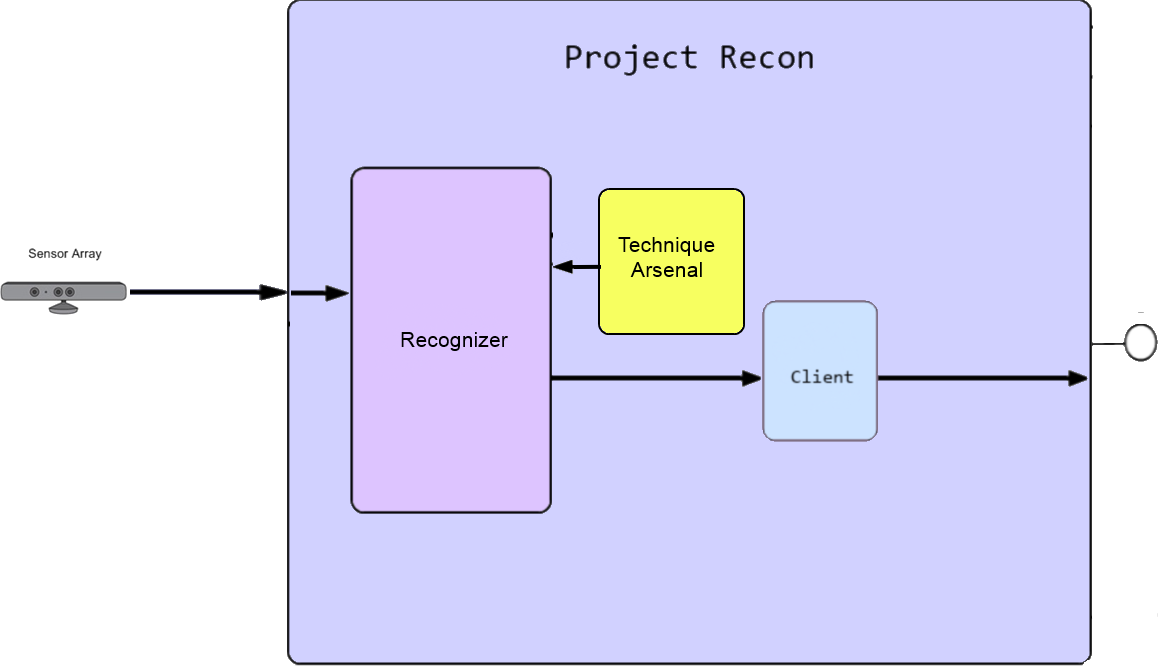
\includegraphics[scale = 0.3] {project_Recon_diagram.png}
\end{frame}

\begin{frame}{Kinect}
\begin{columns}[T]
    \begin{column}{.5\textwidth}
% Your text here
 \begin{itemize}
  \item Four components
   \begin{itemize}
    \item Infrared emitter
    \item Infrared sensor
    \item Color camera
    \item Microphone
   \end{itemize}
  \item Four different streams
  \begin{itemize}
   \item Depth stream
   \item Color stream
   \item Skeleton stream
   \item Audio stream
  \end{itemize}
 \end{itemize}
    \end{column}
    \begin{column}{.5\textwidth}  
% Your image included here
    
\includegraphics[scale=0.25]{kinect.png}
    \end{column}
  \end{columns}
\end{frame}

\subsection{Tools}

\begin{frame}{XNA}
 
\includegraphics[scale = 0.1]{XNA.png}
 \begin{itemize}
  \item Framework based on .NET Compact framework
  \item Created by Microsoft to support game development
  \item Basic platform for the indie games on XBOX Live
  \item Language used is C$^\sharp$
 \end{itemize}
\end{frame}

\begin{frame}{Kinect SDK}

\includegraphics[scale=0.075]{kinectsdk.jpg}
 \begin{itemize}
  \item Is the official SDK for the Kinect system
  \item Manages data streams
 \end{itemize}
\end{frame}

\begin{frame}{Socket Programming}
 \begin{itemize}
  \item Enables Processes to communicate
  \item Used to connect between Project Recon and the Interface
  \item Uses client-server model
 \end{itemize}
\end{frame}

\subsection{Project Requirements}

\begin{frame}{Project Requirements}
 \begin{itemize}
  \item Real time recognition
  \item Robust and Dynamic
  \item Plug in to interface
 \end{itemize}
\end{frame}

\section{Recognition Techniques}
\subsection{Glyphs Method}
%Normal Vector
%problem with kinect
%draw the path that each joint takes and store it in an image

%joints create path shadowing past movements
%each joint has its own exclusive color
%as the user moves glyphs are created
%image of user and glyph
%image of glyph
\begin{frame}{The Challenges in Kinect}
 \begin{itemize}
  \item The user always faces the Kinect
  \item Kinect does not differentiate between facing and not facing
  \item Solution:
   \begin{itemize}
    \item Normalize the skeleton of the user (Always ends up facing)
   \end{itemize}
 \end{itemize}
\end{frame}

\begin{frame}{Normal Vector}
 \begin{itemize}
  \item Create normal between vectors $\vec{r}$, $\vec{c}$, and $\vec{l}$
 \end{itemize}
 \pause
 \centering{$\vec{N}$ = ($\vec{r}$ - $\vec{c}$) $\times$ ($\vec{l}$ - $\vec{c}$)}
 \end{frame}

\begin{frame}{Glyphs Method}
 \begin{itemize}
 \item Rotates the skeleton of the user
  \item Draws the path joints take and  stores it in an image
  \item Each joint will have its own exclusive color
 \end{itemize}
 \centering{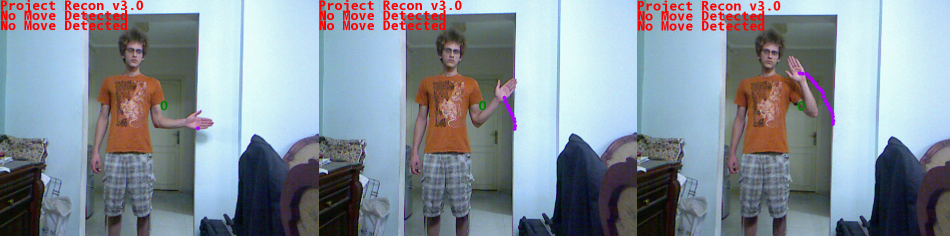
\includegraphics[scale=0.4]{glyphfinal.png}}
\end{frame}
\subsection{Joint Positions Lists}
\begin{frame}{Joint Positions Lists}
 \begin{itemize}
  \item Creates a list (n=30)
  \item The list stores object types StoreGesture (Position, Time Stamp)
 \end{itemize}
 \centering{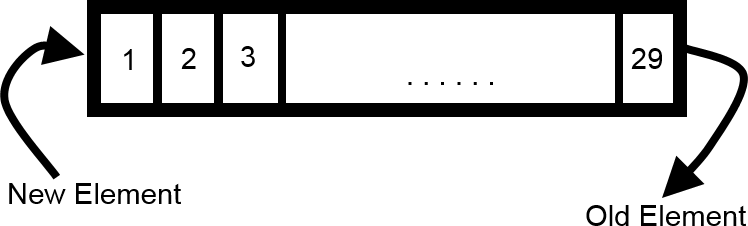
\includegraphics[scale=0.3]{stack.png}}
\end{frame}
\subsection{MCS UK}
\begin{frame}{MCS UK}
 \begin{itemize}
 \item Microsoft Consultant Services UK
 \item Gesture service for Kinect for Windows
 \item The gesture service is written in C$^\sharp$
 \item Similar to the JPL in a manner.
 \end{itemize}
\end{frame}
\begin{frame}{Architecture}
\centerline{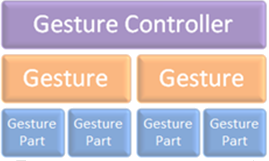
\includegraphics{mcsarc.png}}
\end{frame}
\begin{frame}{Architecture}
\centerline{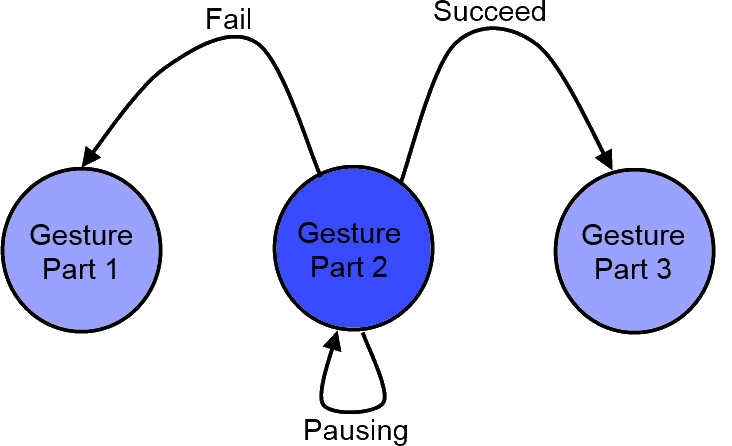
\includegraphics[scale = 0.5]{gesturestate.png}}
\end{frame}
\section{Communication}
\subsection{Communication to the Interface}
\begin{frame}{Communication to the Interface}
\begin{itemize}
 \item Connection is attempted once Kinect is plugged and ready
 \item The interface listens for gestures
 \item User sends gestures with their timestamps
 \item Once connection to the interface falls, program terminates
\end{itemize}
\end{frame}
\subsection{Demonstration}
\begin{frame}{Demonstration}
\centerline{Please Hold for a \texttt{Demonstration}!}

\centerline{[this will only take few minutes]}
\pause
\centerline{\dots I lied}

\end{frame}
\section*{Summary}

\begin{frame}{Summary}
  % Keep the summary *very short*.
  \begin{itemize}
  \item
    \alert{Real time recognition} was accomplished by Kinect's fast streaming.
  \item
    The \alert{Robust and Dynamic} requirement was not fully possible was Kinect has a lot of limitations.
  \item
    \alert{Plugging in to the interface}, was possible through Socket programming.
  \end{itemize}
  
  % The following outlook is optional.
  \vskip0pt plus.5fill
  \begin{itemize}
  \item
    Outlook
    \begin{itemize}
    \item
      Differentiation between facing and not facing(Solved in the new Kinect).
    \item
      Detecting minor movements.
    \end{itemize}
  \end{itemize}
\end{frame}

% All of the following is optional and typically not needed. 
\appendix
\section<presentation>*{\appendixname}
\subsection<presentation>*{Q\&A}
\begin{frame}{Q\&A}
\centerline{Thank you for listening,}
\centerline{floor is open for Q \& A}
\end{frame}
\end{document}


